


  \system, illustrated in Figure \ref{fig:system}, is a processor architecture which aims at providing secure code execution by means of \puf-based authentication of cache lines. The central idea behind \system~is a \puf-Tag (\ptag) Memory, which runs in parallel with the system main memory (Figure \ref{fig:system}). Each entry in the \ptag~Memory stores an authentication code of a cache line generated by a \puf-based device located on-chip.
  
  \begin{figure*}[!ht]
	\centering
	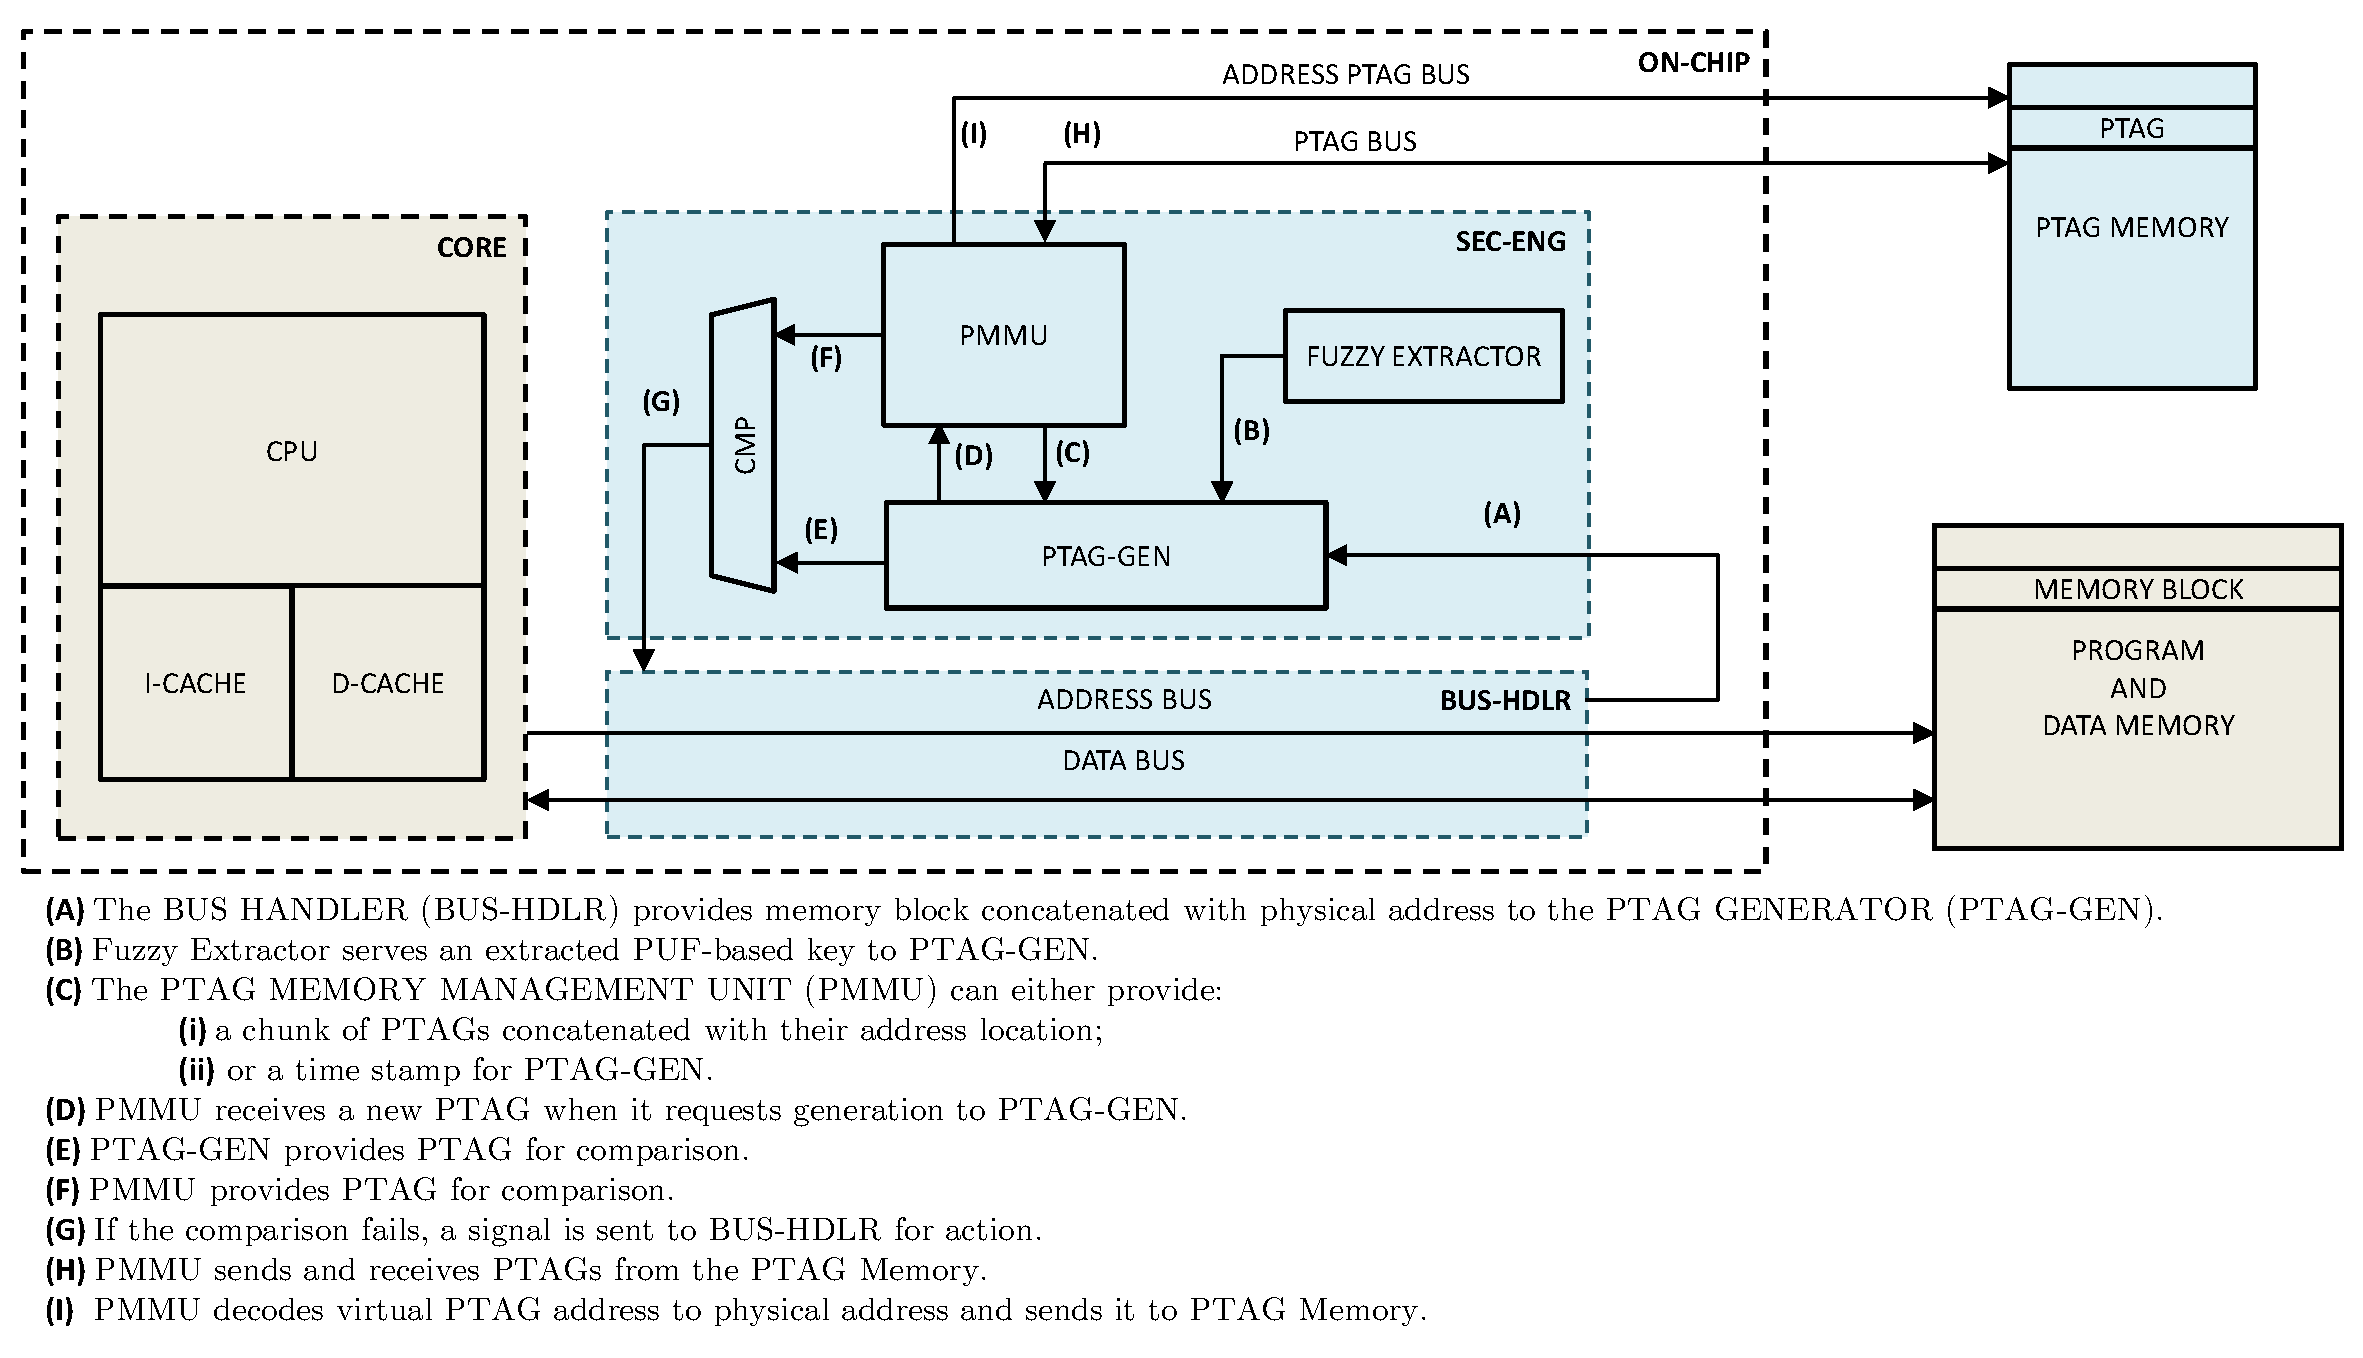
\includegraphics[scale=0.35]{cshia}
%	\vspace*{-12pt} 
	\caption{A system overview of the \system~system.}
%	\vspace*{-9pt} 
	\label{fig:system}
\end{figure*}

  \new{In comparison to traditional architectures, \system~includes two main modifications: The \textit{Secure Engine} (\tagsystem), which includes the \textit{PTAG Generator} (\ptaggen, Figure \ref{fig:ptaggen}); and the \textit{Security-Cache} (\seccache) that controls bus traffic between the processor and the \textit{Memory Controller} (\mctrl). Other two new architectural components are also required to complete the \system~design, the \textit{\ptag~Memory} and the \textit{PTAG Bus}. In a few words, when the processor requires\slash{}sends data\slash{}instructions to the \mctrl, the \seccache~sends the related cache line to the \tagsystem~for computing\slash{}validating its \ptag. Notice from Figure \ref{fig:system} that the \ptag~bus runs in parallel to the system buses, and thus no program can directly read the \ptag~Memory, since neither the processor nor the \mctrl~are aware about the \seccache.}
% 
%   This section is divided in two parts. First, Section~\ref{subsec:ptaggenOpr} details the main operations executed by \system, from the generation of the \ptag~to its validation. Second, Section~\ref{subsec:ptaggenConf} describes the mechanism that extracts the key used to generate the \ptags~and discusses firmware installation.

%   \begin{figure*}[!t]
% 	  \center
% 	  \subfloat[Fuzzy extractor steps during the Enrollment.]
% 	  {
% 		  \includegraphics[scale=0.35]{fuzzy-enrollment.pdf}
% 		  \label{fig:fuzzy-enrollment}	
% 	  }
% 	  \hspace{0.1in}\\		
% 	  \subfloat[Fuzzy extractor steps during the System Reboot.]
% 	  {
% 		  \includegraphics[scale=0.35]{fuzzy-boot.pdf}
% 		  \label{fig:fuzzy-boot}
% 	  }
%   %	\vspace{1in}		
%   %	\hspace{0.2in}		
% 	  \caption{The fuzzy extractor steps for the process Enrollment and System Reboot.}
%   %	\vspace*{-9pt} 
% 	  \label{fig:fuzzy-extractor}
%   \end{figure*}


  \subsection{\ptaggen~Operation}
  \label{subsec:ptaggenOpr}

  \new{The \tagsystem~controls the \ptaggen~based on the information delivered by the \seccache. This information is generated from bus transactions (Memory READ, Memory WRITE and I\slash{}O) between the processor and the memory controller, and which the \seccache~controls. Next, each \ptaggen~action is explained in regard to bus transactions.}
  
      \begin{figure*}[!ht]
	  \centering
	  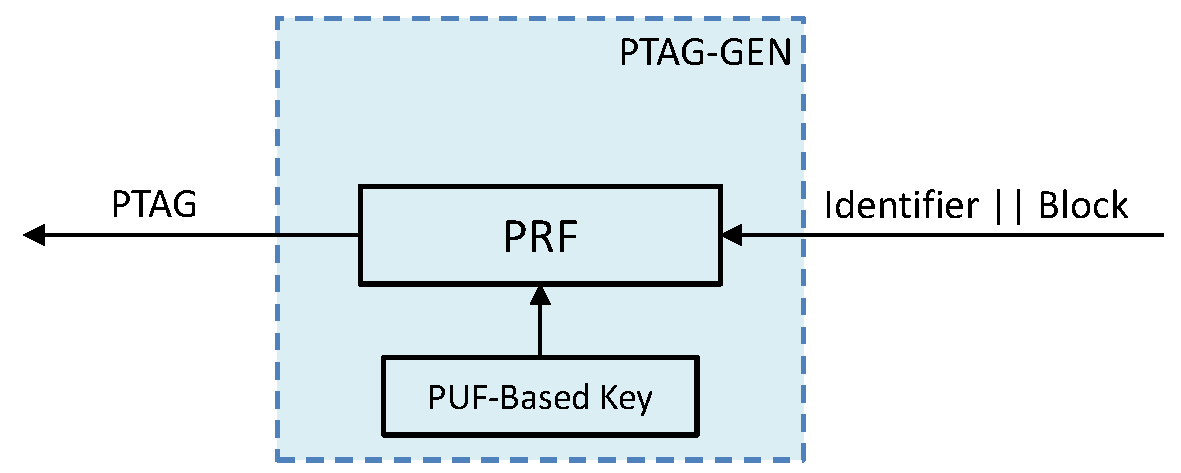
\includegraphics[scale=0.4]{ptaggen}
	  \caption{The \ptaggen~during \ptag~Generation (write) and \ptag~Verification (read) operations.}
  %	\vspace*{-9pt} 
	  \label{fig:ptaggen}
  \end{figure*}
  

	  \subsubsection{\ptag~Generation (memory write)}
	  \label{subsubsec:ptag-generation}
  \new{During a write operation, the \seccache~passes data\slash{}instruction cache lines to the \tagsystem~and the \ptaggen~computes \ptags~and stores it into the \ptag~Memory. A \textit{Pseudorandom Function} (\prf) \cite{Goldreich2004} module is used to generate the \ptag~and takes as input the concatenation ($||$) of the cache line bits and the base address of the cache line provided by the core (see Figure \ref{fig:ptaggen}). In order to ensure uniqueness, the \prf~is configured using a \textit{unique-per-device key}. This key is produced by the intrinsic hardware features of a~\puf. Such authentication tag is specific to the core running that specific cache line, as ~\puf~outputs are dependent on the statistical variations of the manufacturing process, and are unique to each processor~\cite{Katzenbeisser2012}. Hence identical cache lines running on different processors will produce different \ptag~values for the same inputs. Notice that only code in the cache, for which integrity has been ensured, will be able to write to memory.}
  


	  \subsubsection{\ptag~Verification (memory read)}
	  \label{subsubsec:ptag-verification}
  \new{During a read operation, the \seccache~passes data\slash{}instruction cache lines to the \tagsystem~and the \ptaggen~computes \ptags~for verification. As shown in Figure~\ref{fig:ptaggen}, during a read operation the cache line base address produced by the core is appended to the cache line contents read from memory and the result is fed to the \prf~module. The \ptag~produced this way is compared to the PTAG read from memory for equality. If the previously stored \ptag~and the recently computed value do not match, a \textit{Non-Maskable Interrupt} (NMI) is generated to the core (called \ptagnmi), as code\slash{}data integrity may have been violated. As shown in Figure \ref{fig:system}, in order to hide \puf~latency, the data\slash{}instruction is sent to the respective cache (I\$ or D\$) at the same time that \ptag-GEN computes the \ptag~for that cache line and compares it to its \ptag~previously stored into the \ptag~Memory.}

	  \subsubsection{Handling I\slash{}O}
	  \label{subsubsec:io}
  In modern computer systems, I\slash{}O operations store data directly into specific memory regions through DMA mechanism. Thus, it is not possible to trust such memory regions and \system~does not ensure their integrity and authenticity. Software should first perform authentication of I\slash{}O data in a higher abstraction layer and then copy it to secure areas where the \system~can ensure integrity and authenticity.
% 
%   \subsection{\ptaggen~Configuration}
%   \label{subsec:ptaggenConf}
% 
%   \def\fenroll{Figure \ref{fig:fuzzy-extractor} \subref{fig:fuzzy-enrollment}}
%   \def\fboot{Figure \ref{fig:fuzzy-extractor} \subref{fig:fuzzy-boot}}
% 
%   As discussed above, the  \ptaggen~should produce a unique \ptag~for each combination of processor, cache line data and address. To achieve that, the \prf~is configured by means of a \puf~generated key, which is unique to each processor. This key is generated only once and regenerated in each device at turn-on time. Given its simplicity and good statistical metrics~\cite{Katzenbeisser2012}, the \sram~\puf~(\spuf) has been selected for the purpose of this work.
% 
%   One drawback in adopting \spuf~is the additional cost due to its silicon area. To compensate for that, \system~uses the \sram~array of the L1 cache as \spuf~to produce the key. When the processor is turned on, the values of the L1 \sram~cells are set to 0 or 1 according to the physical intrinsic parameters of each L1 \sram~cell. Thus, the \system~key is composed by a set of bits extracted from the \sram~cells of the processor L1 cache at turn-on time.
%   
%   %\subsection*{Enrollment Process}
%   \subsubsection{Enrollment Process}
%   \label{subsubsec:enrollment}
% 
%   Notice that, for a specific processor, the \spuf~bits selected to compose the key should be identical at each \cshia~turn-on time and remain the same during the whole system lifetime. During product setup phase, an \textit{Enrollment} process is run to ensure this. It runs only once, in a controlled environment, and it is composed by three distinct stages described below: Assessment, Extractor Setup, and Firmware Installation.
% 
%   \myparagraph{Assessment:} During this stage, the processor's cache is turned on and off tens of times to find a set $A$ of \spuf~addresses that have stable bits to compose the \prf~key~$k$. This assessment seeks to choose bits that will have a very low bit-flip probability until the end of the hardware lifetime. Although the bits selected this way may not present bit-flips during chip assessment, one cannot assure that flips will never happen as physical parameters of the \spuf~cells can degrade over time. To compensate for that, a Fuzzy Extractor architecture~\cite{Maes2009b, Armknecht2011, Merli2011} is implemented in \ptaggen~to recover the key $k$ in case of some key bits are incorrect when the processor turns on. 
% 
%   \myparagraph{Extractor Setup:}  In this stage, bits are selected from the \spuf, using addresses of $A$, to compose two random words: $r$ and the key $k$. The fuzzy extractor uses them in step 1 as shown in the \fenroll. In step 2, a \bch~encoder receives $r$ and generates codeword $c$. Then, in step 3, the \textit{Key Register} stores $k$ and the fuzzy extractor computes the helper data $h = c \oplus k$. Notice that $h$ can be seen as a one-time encryption of $k$ since the codeword is generated from $r$ that is used only once and then discarded. Furthermore, the codeword encodes no other parameter besides the key. This stage ends with the helper data $h$ and the set of addresses $A$ stored into memory.
% 
%   \myparagraph{Firmware Installation:} In this stage the content of the whole memory is authenticated. First, $h$ and $A$ are authenticated through \ptaggen, generating their corresponding \ptags, which are then stored into the \ptag~Memory. The following authentication steps are for the firmware and the whole memory. This is a one-time procedure which can occur at the solution vendor. In this stage, the  memory controller reads the whole content of the memory (including the firmware), produces their corresponding \ptags~and stores them into the \ptag~Memory.
% 
%   \subsubsection{System Reboot Process}
%   \label{subsubsec:boot}
% 
%   \system~is operational after the Enrollment process finishes and the system is restarted. In this case, a system reboot needs to not only recover the key for \ptaggen, but also avoid leaking any information about the key. The system reboot process also occurs in three stages: \spuf~Recovery, Key Recovery, and Key Validation.
% 
%   \myparagraph{\spuf~Recovery:} At the beginning of the system reboot, the Key Register is in an unknown state. Thus, the only way for \ptaggen~to validate cache lines is to reproduce the original key $k$. At this stage, \tagsystem~recovers $A$, the helper data $h$ and their corresponding \ptags~from the \ptag~Memory (see step 1 in the \fboot). The system now uses $A$ and $h$ to recover $k'$ from the \spuf.
% 
%   \myparagraph{Key Recovery:} Given that there is a non-zero probability that the \spuf~cells flip to different values as the device is turned on, the recovered key $k'$ might not be the same as $k$. To correct $k'$ (step 2), the \tagsystem~computes the $k' \oplus h$, thus generating a codeword $c'$ that differs from $c$ in as many bits as $k$ differs from $k'$. A \bch~decoder is then used to correct $c'$ to $c$, and the operation $c \oplus h$ recovers the original value $k$.
% 
%   \myparagraph{Key Validation:} The recovered key $k$ is stored into the Key Register (step 3, \fboot) and is ready to be used by the \prf~module. Now, before starting the regular operation, the \tagsystem~can validate the helper data $h$ and $A$. If their \ptags~are incorrect the system will stop and generate a \ptagnmi. 
% 
%   Overall, from an architecture perspective, the \emph{main advantages} of the \system~execution model, when compared to other techniques, like~\cite{Suh2005} are: (a) simplicity and ease of integration to current architecture\slash{}programming models without changes in the program toolchain or in the operating system; (b) separated memory buses for improving performance; (c) full-time secure code execution from the system power-on to power-off.
